\documentclass[UTF8]{ctexart}

\CTEXsetup[format={\Large\bfseries}]{section}  
\usepackage{amsmath, amsfonts, amsthm, bm, enumerate, ulem}
\usepackage{epstopdf, graphicx}
\usepackage{algorithm}  
\usepackage{algorithmicx}  
\usepackage{algpseudocode}
\usepackage{booktabs}
\usepackage{mathrsfs}
\usepackage{geometry}
\geometry{scale = 0.8}
\usepackage[colorlinks, linkcolor=red, anchorcolor = blue, citecolor=green]{hyperref}

\floatname{algorithm}{算法}
\renewcommand{\algorithmicrequire}{\textbf{输入:}} 
\renewcommand{\algorithmicensure}{\textbf{输出:}}
\usepackage{listings}
\usepackage{xcolor}
\lstset{
	numbers=left, 
	numberstyle= \tiny, 
	keywordstyle= \color{ blue!70},
	commentstyle= \color{red!50!green!50!blue!50}, 
	frame=shadowbox, % 阴影效果
	rulesepcolor= \color{ red!20!green!20!blue!20} ,
	escapeinside=``, % 英文分号中可写入中文
	xleftmargin=2em,xrightmargin=2em, aboveskip=1em,
	framexleftmargin=2em
}

\theoremstyle{plain}
\newtheorem{thm}{定理}[section]
\newtheorem{lem}[thm]{引理}
\newtheorem{prop}[thm]{命题}
\newtheorem*{cor}{推论}

\theoremstyle{definition}
\newtheorem{defn}{定义}[section]
\newtheorem{conj}{猜想}[section]
\newtheorem{exmp}{例子}[section]

\theoremstyle{remark}
\newtheorem*{rem}{结论}
\newtheorem*{note}{注解}

\DeclareMathOperator*{\argmax}{argmax}
\DeclareMathOperator*{\argmin}{argmin}

\begin{document}
	\setcounter{footnote}{1}
	\title{基于跳过程与统计学习的普适排行榜类产品度量模型}
	\author{程晨\footnote{School of Mathematical Sciences, Peking University, Beijing 100871, China. Email address:
			\href{mailto:moriartycc@pku.edu.cn}{moriartycc@pku.edu.cn}, ID: 1500010714} \quad 陈子恒\footnote{School of Mathematical Sciences, Peking University, Beijing 100871, China. }, \quad 郝天泽\footnote{School of Mathematical Sciences, Peking University, Beijing 100871, China. }}
	\date{}
	\maketitle
	\abstract{
		
		\textbf{关键字:} 
	}
	\newpage
	\tableofcontents
	\newpage
	\section{引言}
	\section{假设}
	在开始阐述我们的模型之前,我们先描述这些模型所依赖的一些基本假设,和所建立的概率模型的空间。
	\paragraph{排行榜} 我们所讨论的排行榜为产品状态集合$\mathcal{P}=\left\{1,2,\cdots,N \right\}$的一个排序,我们将所有排行榜产品构成的集合记为$\Omega_P$,则$\forall \omega \in \Omega_P$,我们就有一个排行榜
	$$
	\omega = (p_1,p_2,\cdots,p_N)
	$$
	\paragraph{产品固有性质} 为了能够度量排行榜类产品的“优劣”,我们假设产品本身有一些固有性质。如果直接定义一个“好坏”的程度,既难以描述和精确定义,又不适合在现实中使用。因此,我们考虑一些能够准确观察到和用统计方法推断的性质,且所有数据都能够用\textbf{用户停留时间}$\tau$和\textbf{用户决策}$a$来确定。对于任意一个产品$i \in \mathcal{P}$,我们假设
	\begin{itemize}
		\item \textbf{用户停留时间$\tau$的分布}。用户停留时间服从一个仅与$i$有关的分布$f_i$,或
		$$
		\tau \sim f_i
		$$
		我们说明这样的假设是合理的。尽管对于每一个不同的用户$u$,其所对应的$f_i^u$可能不同(我们认为一个确定的用户使用同一份产品所用的时间也是一个随机变量)。但考虑所有用户集合$\mathcal{U}$,以及每一个用户$u \in \mathcal{U}$被抽样的概率$p_u$,我们就能得到
		$$
		f_i = \sum_{u \in \mathcal{U}} f_i^u p_u 
		$$
		\item \textbf{用户的决策$a$的可能性}。对于排行榜类产品,用户本身可能有多种感官或心理上的体验,但这些体验并不能被开发者观察和收集到,因此并不是我们所关心的。我们关心的是用户所做的决策,而这些决策将被用来衡量排行榜类产品的好坏。具体来说,根据我们研究的不同排行榜类模型,我们将用户的决策分为
		\begin{itemize}
			\item \textbf{接受(Accepted)}:对于选择型的排行榜,接受表示用户阅读该产品后选择了该产品。
			\item \textbf{放弃(Rejected)}:对于选择型的排行榜,放弃表示用户阅读该产品后放弃了该产品。
			\item \textbf{跳过(Skipped)}:对于选择、投票型的排行榜,跳过表示用户没有阅读该产品就直接跳过。
			\item \textbf{结束(Terminated)}:对于投票型的排行榜,结束表示用户结束了他的阅读过程。
			\item \textbf{投票(Voted)}:对于投票型的排行榜,投票表示用户阅读该产品后进行的决策,具体来说可以有三种
			\begin{itemize}
				\item \textbf{支持(Up vote)}
				\item \textbf{反对(Down vote)}
				\item \textbf{不表态(No vote)}
			\end{itemize}
		\end{itemize}
	\end{itemize}
	\paragraph{用户} 对于用户来说,我们关心他们的停留时间$\tau$和决策$a$。相应的,我们做出这些假设
	\begin{itemize}
		\item $\tau$为指数分布。即$f_i = \mathrm{Exp}(\lambda_i)$。这样的假设是常用且合理的。
		\item 用户群体对于接受、放弃、跳过、结束、支持、反对和不表态分别有基于产品的固有概率$a_i,r_i,s_i,t_i,u_i,d_i,n_i$。
		\item 产品独立性。每个用户使用当前产品时不会受到之前产品的影响,且不考虑个人喜好的因素,即其所做决策的概率完全有产品本身决定。
	\end{itemize}
	
	\section{无跳过的顺序选择模型——Steam探索队列}
	\subsection{模型概述 \& 符号约定}
	我们首先考虑一种最为简单,受约束较多的排行榜类推荐模型——\textbf{无跳过的顺序选择模型}。\textbf{在这个模型中,每一个用户必须依照排行榜的顺序依次阅读有关每一个产品的信息,不能跳过,且必须作出一个选择(我们假设如果到了排行榜队列底端就必须选择最后一个产品)}。这样的模型是基于著名的游戏品台Steam中的探索队列(\ref{modelA_fig_1})功能简化得到的。
	\begin{figure}[H] 
		\centering
		
\includegraphics[width = 12cm]{modelA_fig_1.png}
		\caption{Steam探索队列}\label{modelA_fig_1}
	\end{figure}
	(请在这里添加一段对于Steam探索队列的描述) \\
	
	具体来说,我们给出无跳过的顺序选择模型的定义。
	\begin{defn}\textbf{(无跳过的顺序选择模型)}该模型是一个建立在状态空间为$\mathcal{P} \cup \left\{A\right\}$上的跳过程。其中$A$表示接受状态。其中状态$i$处的指数闹钟参数为$\lambda_i$,且其嵌入链的转移概率为
	\begin{equation}
	\begin{aligned}
	a_{p_N} & = 1 \\
	\bm{P}_{p_i,A}  & = a_{p_i}, \quad 1 \leq i \leq N \\
	\bm{P}_{p_i,p_{i+1}} & = r_{p_i} = 1 - a_{p_i}, \quad 1 \leq i \leq N-1
	\end{aligned}
	\end{equation}
	相应地,该跳过程的速率矩阵可以描述为
	\begin{equation}
	\begin{aligned}
	\bm{Q}_{p_i,A} & = \lambda_{p_i} a_{p_i}, \quad 1 \leq i \leq N \\
	\bm{Q}_{p_i,p_{i+1}} & = \lambda_{p_i} r_{p_i} = \lambda_{p_i} ( 1 - a_{p_i}), \quad 1 \leq i \leq N-1
	\end{aligned}
	\end{equation}
	在图($\ref{modelA_fig_2}$)中展示了具体的模型。该模型可表述为$\mathfrak{A}\left(\bm{\lambda}, \bm{a}, \omega\right)$。
	\end{defn}
	\begin{figure}[H] 
		\centering
		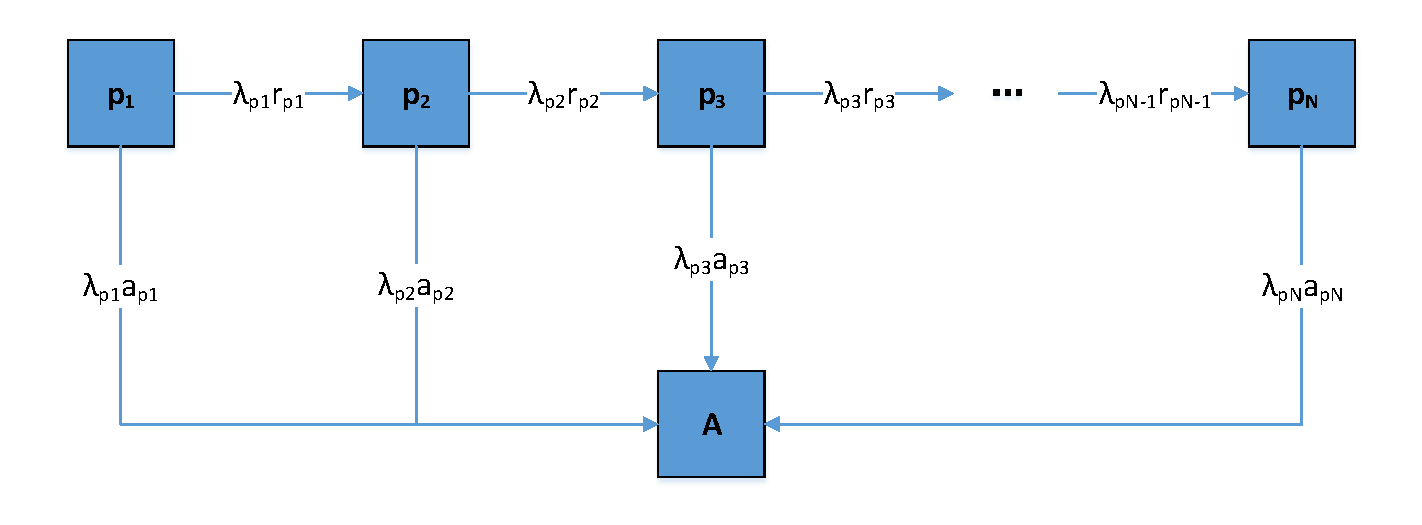
\includegraphics[width = 12cm]{modelA_fig_2.pdf}
		\caption{无跳过的顺序选择模型结构}\label{modelA_fig_2}
	\end{figure}
	(请在这里添加一段对于该模型的感性描述)
	\subsection{度量模型}
	在这样的模型中,我们有理由设置用户找到其接受的产品的时间$\tau_E$为衡量产品优劣的标准。时间越短,那么产品就越有效。而$\tau_E$在对应的随机过程中即为到达状态$E$的首达时,其分布函数可以表示为
	$$
	F_{\tau_E}(t) = e_{p_1}^T \exp(\bm{Q}t)e_{E}, \quad e_i \in \mathbb{R}^{N \times 1}, i \in \mathcal{P}
	$$
	其方差和期望分别为(约定$a_{p_0} = 1$)
	\begin{equation}
	\begin{aligned}
	\mathbb{E} \tau_E & = \sum_{k=1}^N \frac{\prod\limits_{j=0}^{k-1}a_{p_j}}{\lambda_{p_i}} \\
	\mathrm{Var} \tau_E & = \sum_{k=1}^N \left(\frac{\prod\limits_{j=0}^{k-1}a_{p_j}}{\lambda_{p_i}}\right)^2
	\end{aligned}
	\end{equation}
	证明请参见附录。为了综合考虑期望和方差,以及展现出用户对于长队列的不满程度,我们将衡量函数定义为
	\begin{equation}
	\mathrm{Score}_{\mathfrak{A}\left(\bm{\lambda}, \bm{a}, \omega\right)}(x, \alpha) =  \sum_{k=1}^N \left(\frac{\prod\limits_{j=0}^{k-1}a_{p_j}}{\lambda_{p_i}} x^k\right)^\alpha, \quad x \in [0, \infty), \alpha \in [1,2]
	\end{equation}
	
	(请在这里添加一段对于此衡量函数的定性描述,以及合理性分析) \\
	
	当然,由于参数$\bm{\lambda}, \bm{a}$是隐含的,我们需要通过统计推断的方法得到它们,即通过数据得到推断的参数$\bm{\hat{\lambda}}, \bm{\hat{a}}$,然后得到我们的衡量函数
	$$
	\mathrm{Score}_{\mathfrak{A}\left(\bm{\hat{\lambda}}, \bm{\hat{a}}, \omega\right)}(x, \alpha)
	$$
	且$\mathrm{Score}_{\mathfrak{A}\left(\bm{\hat{\lambda}}, \bm{\hat{a}}, \omega\right)}(x, \alpha)$越小,则排行榜产品越好。
	\subsection{统计推断 \& 优化算法}
	对于参数$\bm{\lambda}, \bm{a}$的推断我们使用极大似然估计,即假设第$m$个用户接受了第$p_{k_m}$个产品,前$k_m$个产品的浏览时间分别为$t_{m,i}, 1 \leq i \leq m$,总共有$M$个用户数据被收集,那么似然函数为
	\begin{equation}
	\mathcal{L}\left(\bm{\lambda}, \bm{a}, \omega\right) = \sum_{m=1}^M \ln p_k(\bm{\lambda}, \bm{a}) = \sum_{m=1}^M \ln \left(\left(\prod_{i=1}^{k_m-1}(1-a_{p_i})\right)a_{p_{k_m}}\left(\prod_{i=1}^{k_m} \lambda_{p_i}\right)\exp\left(-\sum_{i=1}^{k_m}\lambda_i t_{m,i}\right)\right)
	\end{equation}
	容易看出此对数似然函数为凸函数,我们使用成熟的凸优化工具(CVX toolbox)可以得到极大似然估计
	$$
	\left(\bm{\hat{\lambda}}, \bm{\hat{a}}\right) = \argmin_{\left(\bm{\lambda}, \bm{a}\right)} \mathcal{L}\left(\bm{\lambda}, \bm{a}, \omega\right)
	$$
	利用推断得到的参数就可以计算衡量函数了。
	\subsection{实验结果}
	\section{带跳过的顺序选择模型——美团外卖}
	\subsection{模型修正 \& 符号约定}
	\subsection{度量模型 \& 统计推断 \& 优化算法}
	\subsection{实验结果}
	\section{带跳过的投票模型——豆瓣、知乎推荐}
	\subsection{模型修正 \& 符号约定}
	\subsection{度量模型 \& 统计推断 \& 优化算法}
	\subsection{实验结果}
	\section{实际产品评价}
	\subsection{两种著名的排行榜产品}
	\subsection{不同情形下的实验比较}
	\section{由此启发得到的基于优化的排行榜算法}
	\section{总结}
	\bibliography{bib}
\end{document}
		
		 